\section{Thermal Phenomena}
    Thermal systems have a \textbf{temperature} and \textbf{thermal contact} allows the system to reach \textbf{thermal equilibrium}, or a common temperature. The \textbf{volume} and \textbf{pressure} of a gas are closely related to temperature.
    \begin{equation*}
        T = \lim_{p \to 0} \frac{p}{p_{tp}}(273.16 K)
    \end{equation*}
    $p_{tp}$ is the pressure of water at its triple point: when ice, steam, and liquid water can coexist in equilibrium. The \textbf{ideal-gas} equation of state relates thermodynamic variables:
    \begin{equation*}
        pV = nRT = NkT
    \end{equation*}
    where $n$ is the number of moles of gas, $N$ is the number of individual gas molecules. $n = N \cross N_A$ where $N_A$ is \textbf{Avogadro's numbers} ($6.23 \cross 10^{23}$). $R$ and $k$ are the \textbf{universal gas constant} (8.314 J/($\text{mol} \vdot \text{K}$)) and \textbf{Boltzmann's constant} ($R \cross N_A$).
    \newline \indent
    Thermodynamic transformations occur when thermodynamic variables change under outside influences. A transformation can either by a \textbf{reversible transformation} (a piston pushed into a cylinder) or an \textbf{irreversible transformation} (gas freely escaping from a container), which are often spontaneous. There are three types of reversible transformations: isothermal, isobaric, and isochoric, in which the temperature, pressure, and volume, respectively, remain fixed.
    \begin{center}
        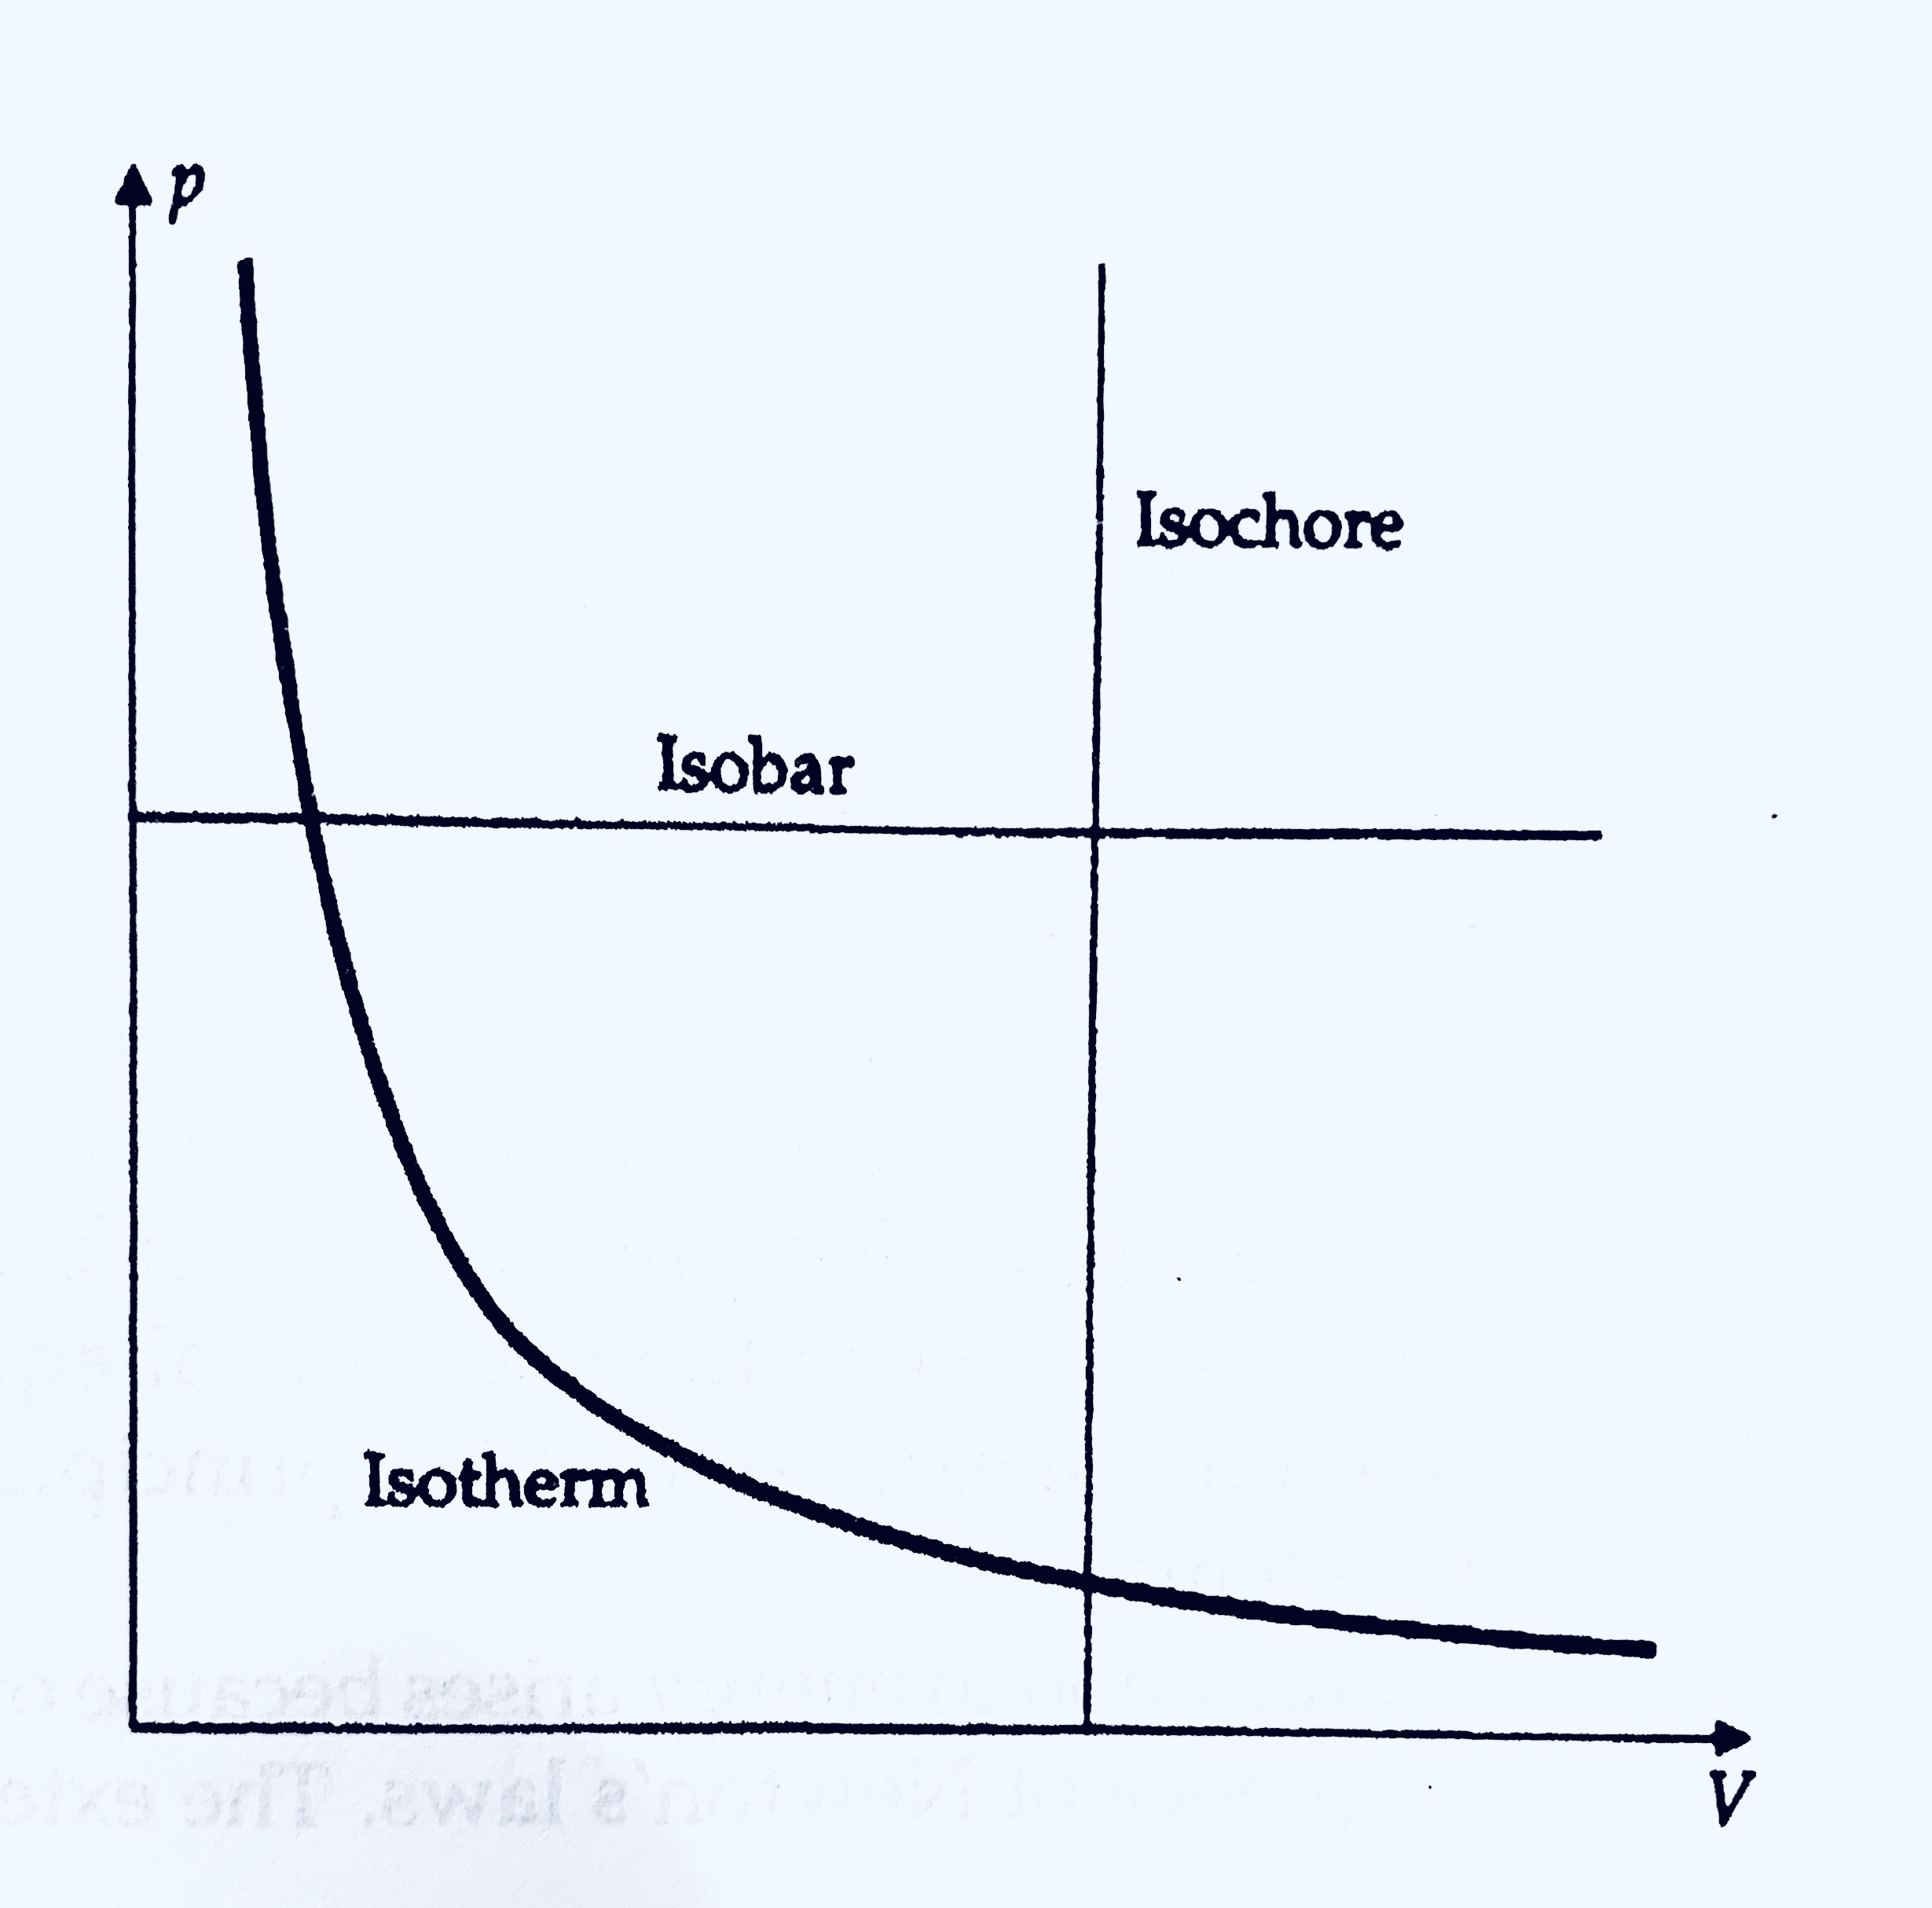
\includegraphics[width=125pt]{pvdiagram.jpg}
    \end{center}
    In the case of a piston being pushed into a cylinder containing gas, we can look at the work done by the gas on the piston. $dW = F\;dx = pA\;dx = p\;dV$, so 
    \begin{equation*}
        W = \int_{V_i}^{V_f}p\;dV
    \end{equation*}
    or the area under a curve of a p-V diagram. This is a path dependent quantity. 
    \newline \indent
    Temperature can also be added through thermal contact: adding heat to the system. The differential amount of heat $dQ$ added is proportional to the temperature change $dT$, so that $$dQ = C \; dT$$ where $C$ is the \textbf{heat capacity}, a quantity that depends on how the temperature change has been made. $C_V$ is when volume is constant. $Q$, heat, is also a path dependent quantity and if no external work is done then heat must be conserved. A transformation with no thermal contact is called \textbf{adiabatic}.
    \newline \indent
    \textbf{Thermal energy} $U$, aka internal energy, is $$dU = dQ - dW$$ where $dQ$ is the heat added to the system and $dW$ is the work done by the system. This is known as the \textbf{first law of thermodynamics}. For constant volume,
    \begin{equation*}
        U(T) = \int dQ - 0 = \int^T C_V \; dT = C_V T
    \end{equation*}
    The \textbf{second law of thermodynamics} states that no engine can be perfectly efficient.
    \begin{equation*}
        \text{maximum efficiency} = 1 - T_c/T_h
    \end{equation*}
    Entropy is a measure of chaos in a system. In an isolated system, entropy has the property that it increases when irreversible processes occur.  The stable equilibrium state is the state of maximum entropy.
    \subsection*{Kinetic Theory}
        Temperature can be understood in terms of the \textbf{kinetic theory of gases}. Consider this situation, gas is applying pressure to a wall. The internal energy of the gas is the sum of all the kinetic energies of the particles ($U = NK_{av}$). We can assume that all the particles are moving at the same speed. 
        \newline \indent
        Now consider a single molecule with initial velocity $\va{v}$ bouncing elastically from the wall with area $A$ in the $yz$-plane. The change in momentum of the particle is $2mv_x$. 
        \newline \indent
        Let $n(\va{v})$ be the distribution function: the number of particles with velocity $\va{v}$ per unit area. Let's look at the molecules with velocities ranging from $\va{v} = (v_x, v_y, v_z)$ to $\va{v} + d\va{v} = (v_x + dv_x, v_y + dv_y, v_z + dv_z)$. $n(\va{v}) d^3\va{v}$ is the number of molecules within this range per unit volume since it is a uniformly random distribution.
        \newline \indent
        For the particle to hit the wall it must be within $v_x dt$ of the wall and it must be in the area $A$. So it must be in the prism with height $v_x dt$ and base area $A$ (the wall).
        \newline \indent
        So the total change in momentum is
        \begin{equation*}
            dp_{tot} = (2mv_x)n(\va{v})d^3\va{v}(v_xdtA) = 2mdtAv_x^2n(\va{v})d^3\va{v}
        \end{equation*}
        \begin{equation*}        
            dF = \frac{dp_{tot}}{dt} = 2mAv_x^2n(\va{v})d^3\va{v}
        \end{equation*}
        \begin{equation*}
            dP = \frac{dF}{A} = 2mv_x^2n(\va{v})d^3\va{v}
        \end{equation*}
        To find total pressure $P$ (for all particles not only in velocity range) we must integrate through all $v_y$, $v_z$, and all $v_x > 0$ (must be going towards wall).
        \begin{equation*}
            P = 2m\int v_x^{2}n(\va{v})d^3\va{v} \text{for all $v_x > 0$} = 2m\frac{1}{2}\int v_x^{2}n(\va{v})d^3\va{v}
        \end{equation*}
        since $v_x > 0$ will occur about half the times since direction uniformly random. 
        \newline \indent 
        Since all directions are uniformly distributed ($n(\va{v}) = n(v)$),
        \begin{equation*}
            \overline{v_x^2} = \overline{v_y^2} = \overline{v_z^2}
        \end{equation*}
        and $v^2 = v_x^2 + v_y^2 + v_z^2$ so on average $v_x^2 = v^2/3$. Since $v$ is a constant for all molecules, it can be taken out of the integral.
        \begin{equation*}
            \int n(\va{v})d^3\va{v} = N / V
        \end{equation*}
        the number of molecules per unit volume since $n(\va{v})$ is for the range from $\va{v}$ to $\va{v} + d\va{v}$ and the integral is for all $\va{v}$.
        \newline \indent
        Using these properties,
        \begin{equation*}
            P = m\int v_x^2 n(\va{v}) d^3\va{v} = \frac{mv^2}{3} \int n(\va{v})d^3\va{v} = \frac{mv^2}{3} (\frac{N}{V}) = \frac{2}{3}K_{av}(\frac{N}{V})
        \end{equation*}
        \begin{equation*}
            PV = nRT = NkT = \frac{2}{3}K_{av}N = \frac{2}{3}U
        \end{equation*}
        \begin{equation*}
            U = \frac{3}{2}NkT \text{ and } kT = \frac{2}{3}K_{av}
        \end{equation*}